
%
% ---- Chapter layout ----
%
% 1) Introduction - 
% 2) 
% ------------------------



\chapter{Biogenic Isoprene emissions in Australia} % Chapter title
\label{BioIsop}


\section{Outline TODO: move into intro?}
  \textbf{Currently this is an outline, TODO: Remove or put into aims.}
  
  %% WHAT we aim to do
  We estimate isoprene emissions in Australia using top-down estimates based on recalculated OMI HCHO measurements and modelled isoprene to HCHO yields.
  These estimates are compared to several campaigns (SPS1, SPS2, MUMBA, Daintree) and used as the new boundary conditions for GEOS-Chem.
  Sensitivity to soil moisture, (maybe) LAI, and satellite AMF calculation is examined and quantified for some scenarios.
  The effect of using these new top down isoprene emissions as the boundary conditions for GEOS-Chem is studied
  Wellness of fit between in-situ (at Wollongong) HCHO, satellite (OMI), and modelled (GEOS-Chem) HCHO is determined with and without updated emissions estimates.
  
  %% HOW it works
  With the vertical columns of biogenic HCHO we can infer the local (grid space) isoprene emissions using effective molar formaldehyde yield (In other continents around 2-3, or 1 in low NO$_X$ conditions) \citep{Palmer2003,Marais2012,Bauwens2016}.
  If we assume there is fast HCHO yield, so that the effect of chemical transport is minimal, and that HCHO and isoprene are at steady states, then we can calculate local yield from our CTM.
  %This yield is derived from both HCHO and isoprene, such as was used by \citet{Millet2006} who produced a molar HCHO yield of 2.3 in north eastern USA.
  Yield is calculated from the modelled slope between isoprene emissions and HCHO total column within each gridbox over Australia, as performed in \cite{Palmer2003}, using modelled values between 1200-1400 LT which is around the overpass time of the OMI.
  This modelled yield is then used in conjunction with the recalculated OMI measurements in order to estimate isoprene emissions.
  To calculate emissions we use a reduced major axis (RMA) regression between modelled average values of the loss rates and total columns, an example is shown in figure TODO: figure with RMA of these over whatever time and space I end up using.
  
%----------------------------------------------------------------------------------------
% Section 1 -- INTRO 
%----------------------------------------------------------------------------------------
\section{Introduction}  
\label{BioIsop:intro}  
  
  One of the most popular emissions inventories for biogenic isoprene, the Model of Emissions of Gases and Aerosols from Nature (MEGAN).
  Global atmospheric studies often use MEGAN along with a chemical transport model (CTM) to examine transport, deposition, and various chemical processes in the atmosphere.
  Emissions of Biogenic Volatile Organic Compounds (BVOCs) including isoprene are often the subject of studies as they are still relatively uncertain, as well as being drivers for imprtant oxidation and pollution events.
  
  (MEGAN) is poorly calibrated for Australian conditions, their emissions of isoprene (C$_5$H$_8$) may be overestimated, especially in the southeast.
  \cite{Muller2008} compared MEGAN against emissions calculated using top down estimates from the GOME2 satellite measurements of formaldehyde.
  \cite{Stavrakou2015} showed that this overestimate may be a factor of 2-3 in January.
  \cite{Sindelarova2014} show how 50\% of the isoprene emissions could be reduced by accounting for lower soil moisture.
  \cite{Emmerson2016} discuss the suitability of MEGAN's isoprene and monoterpene emission factors over southeast Australia, and suggest isoprene emissions are estimated 2-6 times too high.
  They also show that no blanket increase or decrease in emission factors is appropriate for the entire southeast of Australia.
  Satellite based emissions estimates may allow us to improve the models without requiring lots of hard work on calibrating MEGAN to the large data sparse continent of Australia.
  Emissions of monoterpenes (C$_10$H$_16$, two units of isoprene) may also be underestimated in southeastern Australia, which could lead to the unique scenario of neither type of emission dominating VOC chemistry over the forests \citep{Emmerson2016}.
  
  %% Isoprene to HCHO link
  Isoprene has a large impact on the oxidative properties of the atmosphere, as it reacts quickly with the OH radical to form RO$_2$ and then in the presence of NO$_X$ various OVOCs (largely HCHO), SOAs and ozone are formed.
  Isoprene is emitted and enters the atmosphere in the gas phase, where it reacts with various chemicals, forming many new chemicals and reactions at various time scales.
  For more on the pathways and reactions of isoprene in the atmosphere see Section \ref{LR:VOCs:IsopCascade}.
  Formaldehyde is produced with high yields in many of the isoprene reactions, and is often used as a check on how well these reactions are simulated by comparison against in-situ measurements \citep{Marvin2017}.
  
  %% AIMs paragraph
  Here we introduce how uncertain isoprene emissions are over Australia, and discuss literature which shows how the estimates may be too high.
  Section \ref{BioIsop:MethodsAndData} describes the methods, models, and campaign data we use to determine and analyse isoprene emissions.
  The OMI measurements used in this research are recalculated using an updated estimate of HCHO profiles and validated against Wollongong total column measurements. 
  
\section{Data}
  \label{BioIsop:Data}  
  
  \subsection{OMI NO2}
    NO$_2$ measured by OMI is used to check whether NO$_2$ is well represented by GEOS-Chem. 
    OMNO2d is a gridded daily level three product with good satellite pixels averaged into 0.25x0.25$^{\circ}$ horizontally resolved bins.
    See section \ref{BioIsop:Methods:NOx} for how this product was used to check GEOS-Chem calculations. TODO: move this subsection or point to the right area.
  
  \subsection{OMI HCHO}
  
  \subsection{Drought Index}
    The S Precipitation Evapotranspiration Index (SPEI) is a measure of drought using various parameters such as TODO. (\cite{Wang2017}).
    SPEI will be compared against the difference between top-down estimated emissions and MEGAN bottom up estimated emissions. 
    This is used to determine whether there are biases in the MEGAN calculations due to the GEOS-Chem implementation ignoring soil moisture.
    It is downloaded from TODO and holds monthly averaged values at 0.5$^{\circ}$ horizontal resolution.
    When comparing against the emissions estimates this is interpolated linearly onto the same grid as that of GEOS-Chem output at 2x2.5$^{\circ}$.
  
  \subsection{GEOS-Chem output}
    There are various outputs available when running GEOS-Chem, which require understanding in order to compare with observations.
    \begin{description}
      \item[Satellite overpass] is output from averaging over a window of local time for each gridbox. 
        This output allows comparison with satellite measurements, which overpass at the same local time every day.
        The output is in bitpunch.
      \item[HEMCO diagnostics] are the emissions TODO: averaged or instantaneous? in each gridbox, which I've stored for each 3 hours.
        This output is netcdf.
      \item[Tracer averages] are daily or monthly averaged gridbox concentrations.
        This output is bitpunch.
        
    \end{description}
  
\section{Modelling}
  \label{BioIsop:Model}
  
  \subsection{GEOS-Chem simulation}
    \label{BioIsop:Model:GC}
    The GEOS-Chem global atmospheric chemistry model (V10.01) simulates and records up to 66 chemical species (tracers) in the standard run, at 2 by 2.5$^{\circ}$ horizontal resolution, with 47 levels up to the top of the atmosphere (TOA at 0.01~hPa). 
    GEOS-5 meteorological fields from NASA's ...(TODO: ref and note) are used to drive transport and coupled with the chemical module of GEOS-Chem.
    MEGAN is used to determine biogenic emissions for our default GEOS-Chem simulation, with subsequent modifications based on top-down estimates made herein.
    
    Output for an area averaged over 1300 - 1400 local time is saved for comparison and recalculation with satellite overpass records.
    These averages are used to calculate both the GEOS-Chem based AMF, and the modelled background HCHO over the remote pacific which is used in the reference sector correction for OMI column retrievals.
    They are also used to determine isoprene to HCHO yield, after removing days with high biomass burning emissions.
  
  \subsection{CAABA/MECCA simulations}
    \label{BioIsop:Model:CM}
    % Description of CAABA/MECCA
    % TODO: Description of CAABA/MECCA and how it's used.
    
    CAABA (Chemistry As A Boxmodel Application) estimates the chemical concentrations accounting for J-values (JVAL), simplified and parameterised photolysis (SAPPHO) and simplified emission and depositions (SEMIDEP).
    
    CAABA/MECCA has been implemented for various calculations including ozone chemistry throughout the atmosphere in \cite{Zanis2014}.
    The user manual is available online at \url{http://www.rolf-sander.net/messy/mecca/caaba_mecca_manual.pdf}.
  
\section{Methods}
  \label{BioIsop:Methods}
  
  
  
  \subsection{CAABA/MECCA Box model: isoprene source classifications}
    \label{BioIsop:Methods:CM}
    
    % HOW WE WILL USE CAABA/MECCA
    Using CAABA/MECCA to examine isoprene to HCHO yield in specific scenarios allows us to determine what environment may be driving the yield calculated by GEOS-Chem.
    Initially we have three scenarios, grassland, desert, and forest Australia - with each scenario having initial conditions, emission and deposition set as in table TODO:\ref{}.
    Running each scenario with and without a small isoprene injection allows calculation of isoprene lifetimes and HCHO yield for those scenarios.
    
    CAABA runs in a single scenario (or box) with given emissions, depositions, and initial concentrations, allowing the examination of chemistry in a very specific environment to be modelled with high temporal resolution.
    This has been used with an atmospheric chemistry model MECCA (Module Efficiently Calculating the Chemistry of the Atmosphere) which implements tropospheric and stratospheric chemistry for both the gas and the aqueous phases \citep{Sander2005}.
    For our purposes it's worth noting that MECCAs chemical mechanism includes basic O$_3$, CH$_4$, NO$_X$, and HO$_X$ chemistry, as well as non methane hydrocarbon (NMHC) chemistry, considering gas phase, aqueus phase, and heterogenous reactions. \citep{Sander2005}
    For the numerical integration, MECCA uses the KPP software \citep{SanduSander2006}, which takes chemical reactions and their rate coefficients and forms efficient code for integral solutions to the system.
    The combination of the CAABA box model with MECCA module is called CAABA/MECCA and is currently at version 3.
    
    
    %TODO: Description of how scenario yields can be calculated.
    We perscribe parameters values approximating three seperate (and relatively broad) scenarios: forest, urban, and scrubland.
    These parameters are shown in Table \ref{BioIsop:table:CAABAMECCA_Scenarios}!
    The initial concentrations, the influx, (TODO: check this) and the deposition rates of various chemical species or families is perscribed, chemical creation, destruction and deposition rates are determined every X minutes.
    This is done by altering a scenarios file which does not change over the lifetime (TODO: 40 days?) of the model runs.
    For each scenario, two nearly identical model runs are performed, one with an injection of isoprene occuring on (TODO: when/howmuch is this injection).
    The concentrations of isoprene and HCHO for our three scenarios, with and without the isoprene injection, is plotted over time in figure TODO: CAABA/MECCA scenario figures.
    The yield of HCHO from isoprene is then calculated by looking at the difference between each parallel run to determine how much of the injected isoprene transformed into HCHO.
    Isoprene life time can also be calculated using this process, as the time it takes for the extra isoprene to reach $1/e$ of it's initial value.
    
    % CALCULATION OF YIELD
    TODO: Calculations for this (from Luke, double check these and enter them here).
    Calculation of the yield follows a calculation of the theoretical maximum carbon production by the amount of injected isoprene:
    \begin{equation}
    Y_{100} =10^9 \times \frac{C_{PM} E_{inj} D_{inj}}{(N_A H_{PBL})}
    \end{equation}
    Where Y$_{100}$ is the maximum possible carbon yield of isoprene (ppb), $C_{PM}$ is Carbon per molecule (isoprene=5), $E_{inj}$ is the emission rate of injected isoprene (molec cm$^{-2}$ s$^{-1}$), $D_{inj}$ is the duration of injection (s), H$_{PBL}$ is the boundary layer height (cm), and $N_A$ is the Air number density (molec cm$^{-3} \approx 2.5e19$).
    Finding the accumulated increase in HCHO (ppb) from the difference between the perturbed and non perturbed model runs allows calculation of the accumulated extra HCHO (Example: Figure TODO:), which divided by the $Y_{100}$ gives us the isoprene to HCHO atom C yield:
    \begin{equation}
    Y_{HCHO}= \frac{\Delta HCHO_{\text{Accumulated}}}{Y_{100}}
    \end{equation}
    with $HCHO_{\text{Accumulated}}$ being the accumulated enhanced ppb mixing ratio of HCHO.
    
    Figure TODO: shows the accumulated yield for all three scenarios, which each increase towards a limiting value.
    
    \begin{table}[t]
      \caption{Parameters for each scenario used in CAABA/MECCA model runs. TODO: fill these values in}
      %    Parameter | S1, S2, S3
      \begin{tabular}{ c |  c   c   c  } 
        \hline
        Parameter(units) 		 & Forest & Scrublands & Urban\\
        \hline
        Initial concentrations & & & \\
        NO$_X$(molec cm$^{-3}$)		 & low  & low  & high \\
        O$_3$(molec cm$^{-3}$)  & mid & mid & low \\
        HO$_X$(molec cm$^{-3}$) & & & \\
        \hline 
        Influx & & & \\
        NO$_X$(molec cm$^{-3}$ s$^{-1}$)		 & low  & low  & high \\
        O$_3$(molec cm$^{-3}$ s$^{-1}$)  & mid & mid & low \\
        HO$_X$(molec cm$^{-3}$ s$^{-1}$) & & & \\
        \hline
        Deposition rates? & & & \\
        \hline
      \end{tabular}
      \label{BioIsop:table:CAABAMECCA_Scenarios}
    \end{table}
  
  \subsection{Recalculation of OMI HCHO}
    \label{BioIsop:omiRecalc}
    The AMFs for OMI are recalculated using shape factors based on GEOS-Chem HCHO profiles, averaged between 1200 and 1400 local time (LT).
    The method used here largely follows that of \citet{Palmer2001}.
    When comparing satellite observations to a chemical model, recalculation of the satellite AMF using modelled vertical gas profiles removes any bias introduced by differences from the a-priori shape factor to the model.
    The AMF is needed to transform the slant column, as viewed by the satellite, into a vertical column:
    \begin{equation} \label{eqn:AMFratio}
    AMF = \frac{\Omega_s}{\Omega_v} %= \frac{\tau_s}{\tau_v}
    \end{equation}
    where s and v subscripts refer to slant and vertical values, while $\Omega$ represents a column of absorber in molecules cm$^{-2}$.
    
    % HERE I SUMMARISE THE AMF CALCULATION
    The vertical shape factor S$_z$(z) is defined as a normalized vertical number density profile $S_z(z) = \frac{\eta(z)}{\Omega_v}$ where $\eta(z)$ is the number density in molecules m$^{-3}$. 
    The AMF can be expressed as
    \begin{equation} \label{eqn:AMFintwSdz}
    AMF = AMF_G \int_0^\infty w(z) S_z(z) \mathrm{d}z
    \end{equation}
    Where w(z) is the scattering weights describing the sensitivity of the backscattered spectrum to the abundance of an absorber at altitude z.
    It's worth noting that in the OMI satellite product, the provided $\omega(z)$ incorporates the $AMF_G$ term and the equation \ref{eqn:AMFintwSdz} should be implemented without this term if using the satellite $\omega$.
    This is not noted in any of the papers which recalculate the AMF from the OMI product, due to them recalculating the $\omega$ term themselves with a radiative transfer model such as LIDORT.
    
    Two HCHO products are created, both using GEOS-Chem output at global 2 by 2.5$^{\circ}$ horizontal resolution.
    One uses the OMI product's $\omega_z$ and equation \ref{eqn:AMFintwSdz} in order to calculate an AMF.
    While the other uses code provided by Dr. Paul Palmer, with alterations by Dr. Randal Martin, and Dr. Luke Surl to run LIDORT on the satellite slant columns and the GEOS-Chem output in order to calculate an AMF.
    These two calculations are compared over Australia in figure(s) TODO: Map comparison, regression, and time series once AMFpp is working properly.
    The effect of not recalculating the $\omega_z$ is TODO: summarise changes between these calculations.
    
    The AMF calculated using Dr. Palmer's code uses a more strict series of filters, leading to fewer satellite based HCHO columns and reduced coverage over Australia.
    Stricter filtering must be balanced against both coverage and the sensitivity of the AMF determination to recalculating $\omega_z$.
    
  \subsection{Calculation of Emissions}
    \label{BioIsop:Calculation}
   
    % FIRST: outline of what we do
    As is done in \citet{Palmer2003, Millet2006, Bauwens2016}, we assume that HCHO, and Isoprene columns are in a steady state, with no horizontal transport.
    We also assume that isoprene is the only compound enhancing the HCHO levels, which requires that we filter out influence from fires.
    Emissions of precursors are easy to calculate as long as we know the molar HCHO yields (Y$_i$) and effective chemical loss rates (k$_i$):
    \begin{equation}
    \Omega_{HCHO} = \frac{1}{k_{HCHO}}\Sigma_i k_i Y_i \Omega_i = \frac{1}{k_{HCHO}}\Sigma_i Y_i E_i
    \end{equation}
    This works if there is fast HCHO yield, so that the effect of chemical transport is minimal.
    The background HCHO is calculated using measurements in the remote pacific at the same time and latitude.
    Table \ref{BioIsop:Methods:tab_VOCAusYields} shows the average yield calculated for Australia. (TODO: this table and some notes)
    
    %% SLOPE Calculation
    In order to approximate the isoprene to HCHO yields over Australia, GEOS-Chem is run and the slope (S) between modelled tropospheric HCHO columns and emissions of isoprene within each grid box. 
    Figure (TODO: example grid box and regression plot.) shows the regression between emitted isoprene and tropospheric column HCHO, averaged between 1200-1300~LT each day.
    We can infer the local (grid space) isoprene emissions (E$_{isop}$) using effective formaldehyde yield from isoprene ($Y_{isop}$).
    \begin{equation} \label{BioIsop:Calculation:eqn_isop_yield}
    \Omega_{HCHO} = S \times E_{isop} + B
    \end{equation}
    Where \textit{B} is the background HCHO, and $S = Y_{isop}/k_{HCHO}$ is determined monthly as the regression between $\Omega_{HCHO}$ and E$_{isop}$ on daily saved outputs from GEOS-Chem over Australia using 2 by 2.5$^{\circ}$ horizontal resolution. 
    Modeled background emissions can be ignored here as they do not affect the slope calculation.
    Once we have calculated this slope, we use the same formula (Eqn. \ref{BioIsop:Calculation:eqn_isop_yield}) to determine the isoprene emissions.
    By replacing $\Omega_{HCHO}$ and $B$ with OMI based values, $E_{isop}$ is the only unknown.
    
    %% NOTE: Satellite uncertainty bounds for slope calculation
    In several studies OMI satellite HCHO columns are scaled up by up to 40\% to match in-situ measurements TODO:citations.
    Since we don't have enough in-situ data to reasonably scale the satellite columns we instead re-run the calculation with them scaled up by 40\% and consider this as a possible bound on satellite uncertainty.
    Yield and estimated top-down emissions are therefore given an upper and lower bound on satellite based uncertainty through this method.
    
    %% BACKGROUND calculation(s)
    There are a couple of ways to determine the modelled background HCHO concentration, one of which involves running the model with isoprene emissions turned off, which allows us to see exactly how much the modelled isoprene emissions alter each vertical column of HCHO.
    This is effective since we have assumed variation in HCHO columns only depends on isoprene emissions, so our background term is theoretically identical to the emission free simulated HCHO.
    The other way involves looking at HCHO over the remote pacific at matching latitudes and times, which emulates how the background is determined for the measured HCHO.
    These modelled background HCHO concentrations are mostly used for comparison with other datasets.
    TODO: show how these two numbers compare! figure with time series of both backgrounds for Aus, SEAus, and remote ocean.
    
    The $B$ackground from OMI  is determined using the mean column HCHO measured over the remote pacific ocean (180-120$^{\circ}$W).
    TODO: Update the background term to do as follows: For this term we average each month of remote ocean measurements, as well as averaging longitudinally within 180-120$^{\circ}$W, and finally $B$ is estimated at each latitude using $\pm 10^{\circ}$.
    This is gives us a background which is appropriate for any latitude, and is shown in Figure TODO: figure with background region highlighted and a time series of background values.
    When calculating the $E_{isop}$ from our modeled slope with OMI HCHO and background, we end up with negative emissions wherever the OMI HCHO column is less than the OMI background (as $E_{isop} = \frac{\Omega_{HCHO} - B}{S}$).
    These are set to zero, which increases the average by around TODO: X\%.
    The measured background HCHO is the average concentration measured in the remote pacific at the same time.
    
    Figure \ref{BioIsop:Calculation:fig_E_isop_vs_hcho_model_sample} shows the modelled isoprene emissions and column HCHO concentrations along with the RMA regression line, sampled from grid boxes over Australia for January 2005.
    Some affects from the low emissions in grid boxes which are largely oceanic can be seen and are handled by TODO: handle these and document here.
    Due to the low horizontal resolution of GEOS-Chem (2 by 2.5$^{\circ}$, latitude by longitude), calculations from grid boxes on the coast which are largely oceanic need to be discarded as the change in HCHO is not dominated by emissions of isoprene, as is assumed for Eqn \ref{BioIsop:Calculation:eqn_isop_yield}.
    A nested version of GEOS-Chem allows a much better analysis of coastal regions, at 0.25 by 0.3125$^{\circ}$ resolution.
    \begin{figure}[!htbp]
      % Figure from GC_tests.py -> isop_hcho_RMA
      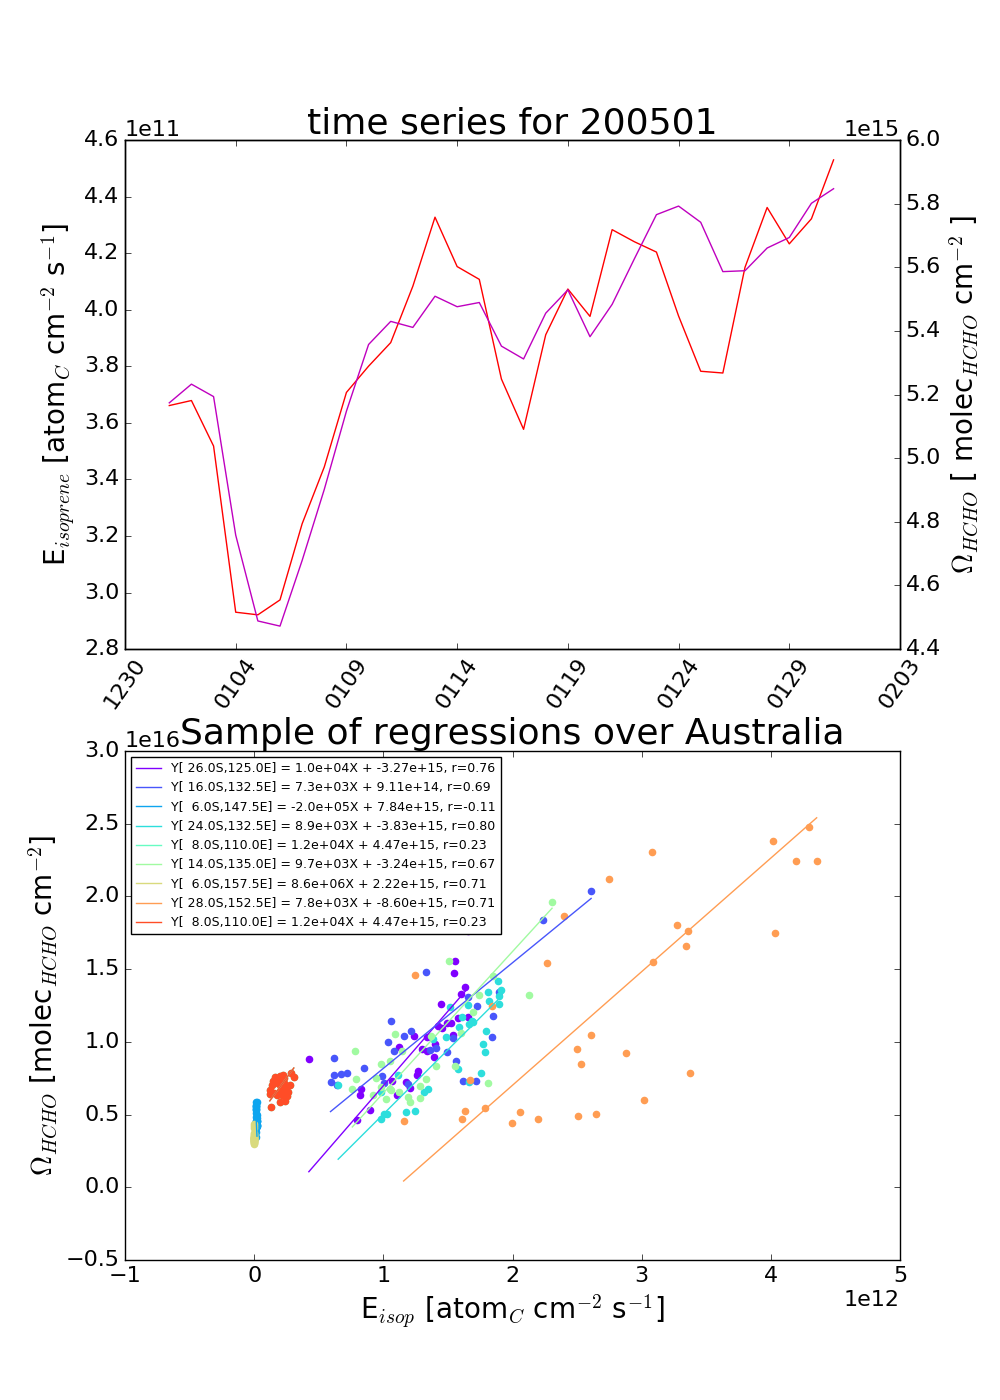
\includegraphics[width=\textwidth]{Figures/Isoprene/E_isop_vs_hcho_series_200501.png}
      \caption{%
        Top panel: isoprene emissions for January, 2005, shown in red, coplotted with tropospheric hcho columns, shown in magenta.
        Both series are daily averages over Australia.
        Bottom panel: (RMA) linear regressions from between emissions of isoprene and tropospheric hcho columns, sampled randomly from the 2$^{\circ}$ by 2.5$^{\circ}$ latitude longitude gridboxes over Australia for the month of January (2005).
      }
      \label{BioIsop:Calculation:fig_E_isop_vs_hcho_model_sample}
    \end{figure}
    
    %TODO: put this into results
    Using this modelled slope at 2$^{\circ}$ by 2.5$^{\circ}$ and applying it to equation \ref{BioIsop:Calculation:eqn_isop_yield} with B and $\Omega_{HCHO}$ calculated using OMI satellite measurements provides a new estimate of isoprene emissions.
    Figure \ref{BioIsop:Calculation:fig_E_isop_200501} shows the emissions calculated this way along with the Emissions output by GEOS-Chem averaged over January, 2005.
    \begin{figure}[!htbp]
      % Figure from Inversion.py -> check_against_MEGAN()
      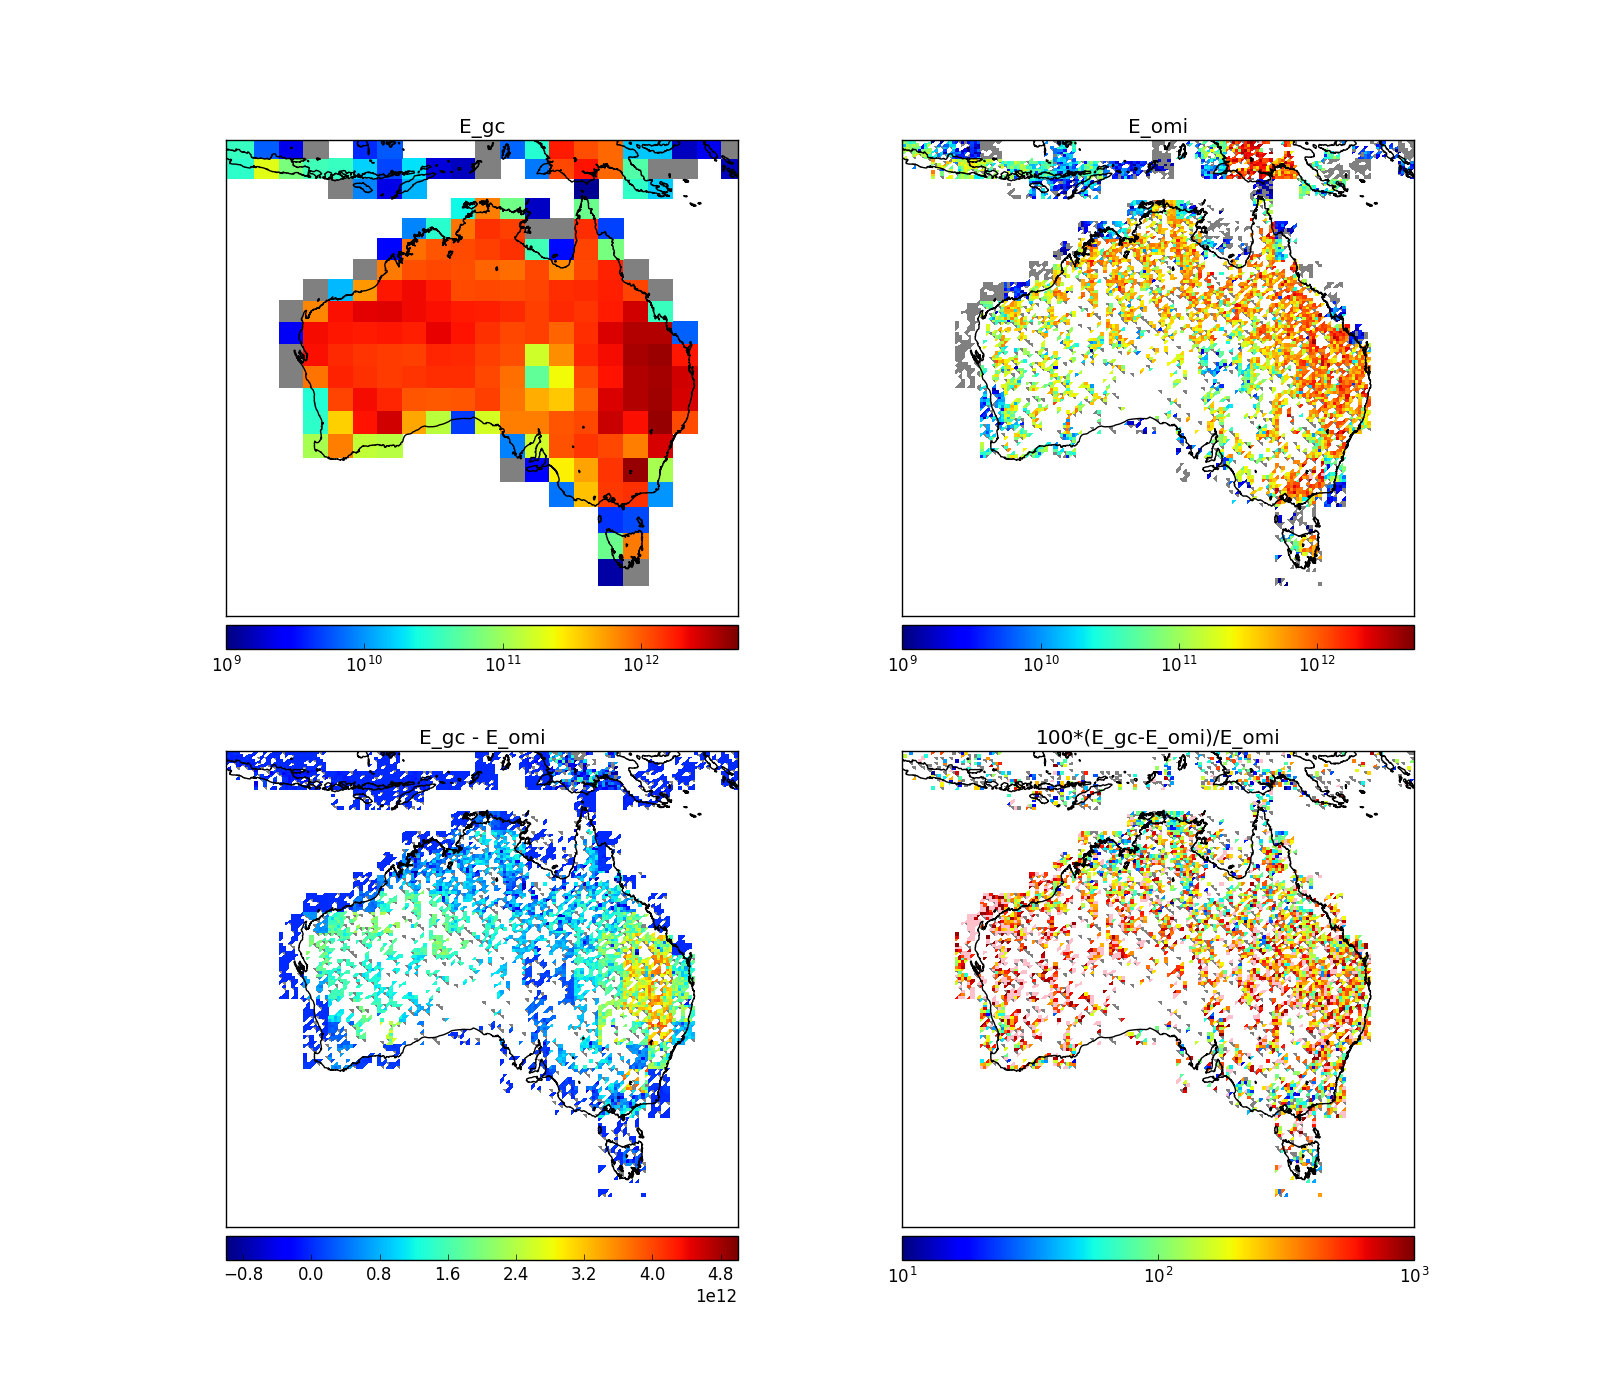
\includegraphics[width=\textwidth]{Figures/Isoprene/E_Comparison.png}
      \caption{%
        Top row is isoprene emissions for the month of January, in 2005, from GEOS-Chem and estimated from OMI respectively.
        Bottom row shows the absolute and relative differences between the two.
      }
      \label{BioIsop:Calculation:fig_E_isop_200501}
    \end{figure}
  
  \subsection{Emisions drivers}
    Calculated yields of HCHO can be classified using a box model which approximates specific environments, as described in Section \ref{BioIsop:CabbaMecca}.
    TODO: A table of different factors affecting emissions for three scenarios; urban, forest, shrublands is given in Table XX.
    The calculated yields for these scenarios is based on the CAABA/MECCA box model (described in Section \ref{BioIsop:CabbaMecca}) TODO: compare scenarios yields and show map of Australia with mapped closest scenario(one colour for each scenario, contourf).
    
  \subsection{HCHO Products and yield}
    \label{BioIsop:Methods:HCHOYield}
    Australian forests are strong emitters of both isoprene and monoterpenes, which go on to form various products including secondary organic aerosols, oxygenated VOCs (OVOCs), ozone, OH, and HO$_2$.
    This production occurs over several steps, yields are often classed into at least two categories.
    First generation yield refers to the amount of HCHO produced per unit isoprene consumed by initial oxidation, total yield (sometimes molar yield) refers to time dependent yield of HCHO over multiple oxidation stages \citep{Wolfe2016}.
    \citet{Wolfe2016} define prompt yield as the change in formaldehyde measurement per unit change in initial isoprene emissions.
    Some argue that isoprene emissions are overestimated, due to the fact that they are based on relatively few measurements of isoprene emission factors \citep{Winters2009, FortemsCheiney2012} TODO: read and cite paper mentioned in Fortems.
    Recently \cite{Emmerson2017} showed that MEGAN estimates 3-6 times too much isoprene emissions, and 4 times too little monoterpenes when compared against 4 (relatively small scale) measurement campaigns in southeastern Australia.
    
    Isoprene production of HCHO depends on several factors, importantly NO$_X$ levels have a direct effect on the fate of VOCs in the atmosphere.
    At higher NO mixing ratios (at least a few hundred pptv), organic peroxy radicals (RO$_2$) react mostly with NO. 
    At low NO (less than 10's of pptv), reaction with HO$_2$, other RO$_2$, and isomerization dominate the fate of RO$_2$.
    In low NO$_X$ environments, reported HCHO yields from isoprene are from XtoY\%, while in high NO$_X$ environments this value is XtoY\% TODO: these values from table.
    For monoterpenes the yields are around X, Y\% for low, high NO$_X$ respectively.
    Emissions and yields for various species including some terpenes can be seen in table \ref{BioIsop:Methods:tab_VOCAusYields}.
    \citet{Wolfe2016} determine that going from NO$_X = 0.1$ to $2.0$ ppbv triples the prompt yield of HCHO, from 0.3 to 0.9 ppbv ppbv$^{-1}$ due to isoprene, while the background HCHO doubles.
    They determine prompt yield as the change in HCHO per change in ISOP$_0$, using $[ISOP]_0=[ISOP]\exp(k_1[\mathrm{OH}]t)$; where $k_1$ is first order loss rate.
    This effectively relates HCHO abundance with isoprene emission strength.
    %TODO:and finish Wolfe2016 discussion paper for yields
    %TODO:go through atkinsonarey2003
    
    NO$_2$ measured by OMNO2d gives us a daily mid-day measurement which we can compare to output from GEOS-Chem to determine how well the model does at simulating NO$_2$.
    This is also done in \cite{Travis2016}, as a way to examine model bias in ozone (potentially due to NO$_2$ bias) over the USA.
    
    
    Looking at Australian emissions from running GEOS-Chem and using yields provided by XYZ (TODO other table), we see that Australia may be more or less likely to do something TODO: this comparison sentence would be good to tie up tables and be copied to conclusions.
    
    Conversions between HCHO per unit C yield and molar \% yield from species X given by the equation $ Y_{molar \%} = 100 \times C_X \times Y_{HCHO per unit C} $, where $C_X$ is how many Carbon are within species X (5 for isoprene, 10 for monoterpenes, etc...).
    For instance a 200\% molar yield of HCHO from isoprene implies 1 Mole of C$_5$H$_8$ becomes 2 Mole HCHO which is a 0.4 HCHO per unit C yield.
    
    TODO: Fill out this table
    \begin{table} \begin{threeparttable}
      \caption{HCHO yields from various species averaged over Australia during Summer.}
      \begin{tabular}{ | c  c  c  c  c | }
        \toprule
        \textbf{Species}   & \textbf{Emissions$^a$}& \textbf{Lifetime$^b$}& \textbf{HCHO Yield$^c$} & \textbf{HCHO production$^d$\%}
        \\                 & (Tg C per month)      &                      & (per C reacted)         &         \\
        \midrule
        Isoprene           & Y                     & n minutes            & 0.x                     & 10       \\
        $\alpha$-Pinene    & Y                     & n minutes            & 0.x                     & 10       \\
        $\beta$-Pinene     & Y                     & n minutes            & 0.x                     & 10       \\
        HCHO               & Y                     & n minutes            & 1.0                     & 10       \\
        \bottomrule
      \end{tabular}
      \begin{tablenotes} 
        \item a: Calculated using GEOS-Chem emissions over Australia in January 2005.
        \item b:  
        \item c: 
        \item d: Production determined by dividing emission*yield by the sum of all VOC emissions*yields. 
      \end{tablenotes}
      \label{BioIsop:Methods:tab_VOCAusYields}
    \end{threeparttable} \end{table}
    
    % yields from Atkinsen2003
    %isoprene
    %0.63 0.10 Tuazon and Atkinson (1990a)
    %0.57 0.06 Miyoshi et al. (1994)
    % a-pinene
    %0.23 0.09 Noziere et al. (1999a)
    %0.19 0.05 Orlando et al. (2000)
    % b-pinene
    %0.54 0.05 Hatakeyama et al. (1991)
    %0.45 0.08 Orlando et al. (2000)
    
    Yields table looking at literature provided yields of HCHO.
    % molar HCHO yield per unit carbon equal to HCHO molar percent yield(per carbon)? or some conversion?
    % TODO: ask steve about ppbv ppbv^-1 ??
    
    \begin{table} \begin{threeparttable}
      \caption{ HCHO yields from various species, and lifetime against oxidation by OH. }
      \begin{tabular}{  l  l  l  l  l  }
        \toprule
        Species    & HCHO Yield    & Life vs OH   & NO$_X$ background & Source   \\
                   & (molar \% )   &              &                   &          \\
        \midrule 
        Isoprene	& 315$\pm$50      &            & High          & a        \\ 
                  & 285$\pm$30      &            & High          & a        \\ 
                  & 225             & 35 min     & High          & b        \\ % Done
                  & 150             &            & Low           & b        \\ % Done
                  & 150             &            & Low           & d        \\
                  & 450             &            & High          & d        \\
                  & 235             &            & 1~ppbv        & e        \\
                  & 150             &            & 0.1~ppbv      & e        \\
        $\alpha$-Pinene & 28$\pm$3        &        & Low                & c        \\ 
                        & X$\pm$3         &        & X                  & d        \\ 
                        & 230$\pm$90      &        & High        & a        \\ 
                        & 190$\pm$50      &        & High        & a        \\ 
                        & 19              & 1 hour &              & b        \\ % Done
                        & 210             &        & 1~ppbv        & e        \\
                        & 70              &        & 0.1~ppbv      & e        \\
        $\beta$-Pinene  & 65$\pm$6        &        & Low           & c      \\ 
                        & X$\pm$3         &        & X             & d      \\ 
                        & 540$\pm$50      &        & High          & a     \\ 
                        & 450$\pm$80      &        & High          & a      \\ 
                        & 45              & 40 min &              & b      \\ % Done
        Methane 	      & 100             & 1 year  &             & b     \\ 
        Ethane          & 180             & 10 days &             & b     \\ 
        Propane         & 60              & 2 days  &             & b     \\ 
        Methylbutanol   & .13(per C)    & 1 hour  &             & b     \\ 
        HCHO            & 100             & 2 hour  &             & b     \\ 
        Acetone         & .67(per C)      & 10 days &             & b     \\ 
        Methanol        & 100             & 2 days  &             & b     \\ %Done
        \bottomrule
      \end{tabular}
      \begin{tablenotes} % \item makes new lines
        \item a \citet{AtkinsonArey2003}: Table 2, Yield from Isoprene reaction with OH, two values are from two referenced papers therein.
        \item b \citet{Palmer2003}: lifetimes assume [OH] is 1e15 mol cm$^{-3}$.
        \item c \citep{Lee2006}: Calculated through change in concentration of parent and product linear least squares regression.
        Estimates assume 20$^\circ$~C conditions.
        \item d \citet{Wolfe2016}: ``prompt yield'': change in HCHO per change in ISOP$_0$.
        $[ISOP]_0=[ISOP]\exp(k_1[\mathrm{OH}]t)$; where $k_1$ is first order loss rate.
        Effectively relates HCHO abundance with isoprene emission strength
        \item e \citet{Dufour2009}: One-day yields from oxidation modelled by CHIMERE, using MCM reference scheme.
        \item f Calculated using PTR-MS and iWAS on SENEX campaign data.
      \end{tablenotes}
      \label{BioIsop:Methods:tab_VOCLiteratureYields}
    \end{threeparttable} \end{table}
  
  
  \subsection{Accounting for smearing}
    \label{BioIsop:Methods:Smearing}
    
    Accounting for transport of the precursors is important, especially in low NO$_X$ conditions in which isoprene has a longer lifetime (days).
    When estimating emissions of isoprene using one of its products, it is often assumed that isoprene has a short lifetime, however when low NO$_X$ environments (which are prevalent in the Australian outback) this assumption can be wrong.
    Smearing (sometimes called spatial smearing) is a measure of how much formaldehyde (the product) was created from isoprene (the precursor) emissions in a different grid box.
    Smearing has been measured in order to account for this uncertainty in various works \citep{Martin2003,Palmer2003,Millet2006,Marais2012,Barkley2013,Zhu2014,Wolfe2016}, often implementing the method designed in \cite{Palmer2003}.
    
    
    Horizontal transport complicates estimation of precursor emissions, as the smearing length scale which increases beyond our gridbox size.
    The smearing length scale; the distance travelled downwind (L$_{d,i}$) by a precursor (i) before becoming HCHO can be estimated using:
    \begin{equation*}
      L_{d,i} = \frac{U}{k_i - k_{HCHO}} \ln{ \left( \frac{k_i}{k_{HCHO}} \right) }
    \end{equation*}
    where U is wind-speed.
    \citet{Palmer2003} further define a smearing length scale: L$_{s,i}$ as the distance downwind where a fraction (1 - $1/e$) of the precursor is completely transformed into HCHO.
    This equation uses the initial VOC column concentration ($[VOC]_0$) at the point of emission and mass balance equations as follows:
    \begin{equation}
    \frac{1}{k_{HCHO}-k_i} \left( k_{HCHO} \exp{ \left[ \frac{-k_i L_{s,i}}{U} \right]} -k_i \exp{ \left[ \frac{-k_{HCHO} L_{s,i}}{U} \right]} \right) = \frac{1}{e} 
    \end{equation}
    with limiting values L$_{s,i} \rightarrow U/k_i$ for $k_i << k_{HCHO}$, and L$_{s,i} \rightarrow U/k_{HCHO}$ for $k_{HCHO} << k_i$.  
    
    TODO: calculation of smearing
    Similarly to smearing sensitivity calculations in \cite{Marais2012}, we run GEOS-Chem with isoprene emissions halved, then calculate $\hat{S} = \frac{\Delta \Omega_{HCHO}}{\Delta E_{Isop}} $, where $\Delta$ represents the monthly mean departure over 1300-1400LT from default run values.
    This allows us to determine which gridboxes are disproportionately affected by emissions from non-local sources.
    Large smearing values can be seen near many coastlines as the Emissions are very low, which makes transported isoprene relatively more important in these gridboxes.
    
    TODO: Plots of S hat showing worst smearing affected areas per season.
    
    
\section{Results}
  
  \subsection{Emissions affect on GEOS-Chem}
    We interpolated or something (TODO) the emissions over Australia into the inventories used by GEOS-Chem which reduced the emissions by X\% per year (over Australia).
    The resulting simulation output shows that HCHO was reduced by X\%, although if we boost monoterpenes by X\% where the isoprene emissions were lowered then 
  
  \subsection{Emissions comparisons}
    
    Some global numbers (TODO: where do I throw these?)
    \citet{Guenther2012} Estimate global biogenic isoprene emissions at roughly 535\tgpyr, using MEGAN.
    \citet{Sindelarova2014} Estimate around 594\tgpyr using MEGAN with MACC, showing isoprene as 69.2\% of the total BVOC emissions, with monoterpenes at 10.9\tgpyr (10.9\%).
    They show 41\tgpyr decrease in Australia when introducing soil moisture parameterisation.
    
    
    When comparing the GEOS-Chem (which runs MEGAN) emissions to those calculated using our top-down inversion, we see a decrease over TODO: locations and seasons.
    TODO: table or figure showing summary of isoprene emissions changes over the whole of our time domain.
    The 'Scaled Satellite' column refers to the calculations when using the 40\% scaled up OMI HCHO columns. %TODO: make table, add that column
    This can be considered as a boundary on satellite based HCHO column uncertainty.
    
    One set of data from the Daintree rainforest in Queensland exists (TODO: summary from P. Nelson).
    Although the data set lies outside our run times, as it was measured in TODO(runtime), we compare against the seasonal average of our GEOS-Chem output for the matching months (TODO: name the months).
    This is done for both GEOS-Chem output and our recalculated isoprene emissions.
    When compared against GEOS-Chem output we see TODO.
    When compared against recalculated emissions we see TODO.
    
    TODO: Figure showing campaign data against model and recalculated emissions over region for averaged months and eventually different resolutions.
    
    %As is done in \cite{Emmerson2016}, 
    We examine the affect of decreased isoprene emissions on the correlation between modelled and satellite based HCHO columns.
    Figure TODO: shows the regressions between GEOS-Chem tropospheric column amounts of HCHO and satellite columns for two runs of GEOS-Chem: a) using standard MEGAN emissions, b) using our updated emissions.
    
    
  
% Extras for potential paper output 
%  
%  \authorcontribution{}
%  \competinginterests{The authors declare that they have no conflict of interest.}%
%  \textit{Data availability.} All GEOS-Chem model output is available from the authors upon request.
%  %\disclaimer{disclaimer}
%  \begin{acknowledgements}
%    This research is supported by an Australian Government Research Training Program (RTP) Scholarship.
%  \end{acknowledgements}
  